\documentclass[version = 3.00]{scrreprt}

%%%%%%%%%%%%%%%%%%%%%%%%%%%%%%%%%%%%%%%%%%%%%%%%%%%%%%%%%%%%%%%%%%%%%%%%%%%%%%%
% To create the final version, uncomment the line containing \finaltrue
\newif\iffinal
\finalfalse
% \finaltrue


%%%%%%%%%%%%%%%%%%%%%%%%%%%%%%%%%%%%%%%%%%%%%%%%%%%%%%%%%%%%%%%%%%%%%%%%%%%%%%%
% Packages & Options

\usepackage[utf8]{inputenc}
\usepackage[T1]{fontenc}
\usepackage[ngerman]{babel}
\usepackage{microtype}
\usepackage{lmodern}
\usepackage{graphicx}
\usepackage{hyperref}
\usepackage{booktabs, longtable, tabu}
\usepackage{enumitem}
\usepackage{xparse}

\iffinal
  % Hide todos in the final version.
  \usepackage[final, obeyFinal]{todonotes}
\else
  \usepackage[ngerman, textsize=footnotesize]{todonotes}
\fi

\iffinal
  % Don't show overfull paragraphs in the final version.
\else
  % This option helps finding paragraphs which are wider than linewidth by
  % drawing a black bar on the right side.
  \KOMAoption{draft}{true}
\fi


%%%%%%%%%%%%%%%%%%%%%%%%%%%%%%%%%%%%%%%%%%%%%%%%%%%%%%%%%%%%%%%%%%%%%%%%%%%%%%%
% Custom commands & adjustments

% Images go into the img/ folder.
\graphicspath{{img/}}

% Commands to indicate missing parts.
\newcommand\missingChapter[2][]{\todo[inline, #1]{\thechapter{} „#2“ schreiben}}
\newcommand\missingSection[2][]{\todo[inline, #1]{\thesection{} „#2“ schreiben}}
\newcommand\missingSubsection[2][]{\todo[inline, #1]{\thesubsection{} „#2“ schreiben}}

% Decrease the font size slightly from \Large to fit all names in two lines.
\addtokomafont{author}{\large}

% Decrease space between table caption and the table's top-rule.
\setlength{\abovetopsep}{-0.8em}

% Spacing between table rows.
\renewcommand\arraystretch{1.3}

% Macros for creating and referencing IDs of actions, objects etc.
%
% The intresting macros defined here are
%   * \StartId{prefix}
%   * \defid[label]{title}, \defid{title}
%   * \refid{prefix:label}
%
% See README.md for an explanation.
\makeatletter
\newcounter{gdd@ids}
\NewDocumentCommand\StartId{m}{%
  \setcounter{gdd@ids}{0}%
  \xdef\gdd@idprefix{#1}}
\NewDocumentCommand\defid{o m}{%
  \ifx\gdd@idprefix\undefined%
    \PackageError{GDD}{Please use \StartId before using \defid}{}%
  \else%
    \leavevmode%
    \refstepcounter{gdd@ids}%
    \IfNoValueTF{#1}{}{\label{gdd-\gdd@idprefix:#1}}%
    \gdd@idprefix\thegdd@ids: #2%
  \fi}
\NewDocumentCommand\refid{>{\SplitArgument{1}{:}} m}{%
  \expandafter\gdd@refformat#1\relax}
\newcommand\gdd@refformat[2]{%
  \IfNoValueTF{#2}
    {\PackageError{GDD}
        {The argument to \refid should be {prefix:label}}
        {It seems you forgot the prefix before the label.}}
    {\hyperref[gdd-#1:#2]{#1\ref*{gdd-#1:#2}}}}
\makeatother


\begin{document}

\title{Spielname\todo[noline]{Das Spiel braucht einen Namen}}
\author{%
  % Sorted alphabetically by last name.
  Melissa Hägle,
  Zacharias Häringer,
  Johannes Mannhardt,\\
  Maximilian Nazarati,
  Jens Rahnfeld,
  Zo\"e Schaaff,
  Janek Spaderna}
\subject{Gruppe 09}
\publishers{Tutor: Daniel Lux}
\maketitle


\tableofcontents
\addcontentsline{toc}{chapter}{Inhaltsverzeichnis}


\iffinal
  % Hide the list of TODOs in the final version.
\else
  \listoftodos
  \addcontentsline{toc}{chapter}{TODOs}
\fi

% FIXME: When this is activated it is quite obvious that for some reason not
% all table numbers are used but some are skipped, e.g. 4.1, 4.2, 4.4, 4.6
% But why?
% \listoftables


%%%%%%%%%%%%%%%%%%%%%%%%%%%%%%%%%%%%%%%%%%%%%%%%%%%%%%%%%%%%%%%%%%%%%%%%%%%%%%%
% Main Content starts here

\chapter{Spielkonzept}

\section{Zusammenfassung}

% Hier ist ein kurzer einleitender Text evtl. in Verbindung mit einem Bild
% gefragt. Ziel ist es, das zu erstellende Spiel in kurzen Sätzen zu erklären
% und die Grundidee zu erläutern. Für die Zusammenfassung kann man sich an den
% "Klappentexten" auf der Rückseite von Spieleverpackungen orientieren. Der
% Text darf als einziger im GDD auch reißerisch und dramatisch sein (abgesehen
% vom Screenplay).

\textit{Kernel Panic!} ist ein a-Mazing Tower Defense Spiel.
Dein Supercomputer wird von einem fießen Hacker angegriffen, der versucht deinen Akku in die Knie zu zwingen.
Also handle schnell und baue dir eine geschickte „Firewall“ auf bevor dein Rechner zwangsweise in den Ruhezustand versetzt wird! Plündere dazu dein Hardware-Lager und versperre deinem Angreifer mit defekten Geräten den Weg. -- Doch er wird keine Ruhe geben, bevor du nicht besiegt bist.

Zum Glück hast du Connections zu einem russichen Hacker-Kollektiv, das dir Trojaner, Viren und Co verkaufen kann. Vergeude keine Zeit und schicke in Upload-Wellen deine eigenen Bug-Armeen los, um den Gegner mit seinen eigenen Waffen zu schlagen.

Mit der Zeit sammelst du wichtige Erfahrungen und kannst so deine Angriffe wie auch deine Verteidigung stetig verbessern. Aber mach schnell, denn auch dein Gegner ist auf Upgrades aus und könnte sie dir wegschnappen.


\section{Alleinstellungsmerkmal}

% Was hebt dieses Spiel von der Masse ab? Wodurch versucht man, den Spieler
% (und den Kunden) zu begeistern? Das Alleinstellungsmerkmal ist das Merkmal
% des Spiels, welches es einzigartig macht. Ein Alleinstellungsmerkmal kann
% sowohl ein Feature, als auch ein gesamtes Konzept des Spiels sein.

\textit{Kernel Panic!} ist eine Mischung aus Mazing Tower Defense und MOBA.
Angriff und Verteidigung finden dabei getrennt auf zwei Lanes statt.
Zusätzlich zu den -- für Tower Defense Spiele -- üblichen Einheiten kann man, durch gezielt kontrollierbare „Helden“, seine Angriffsstrategie weiter verfeinern.

Außerdem gibt es ein geteiltes Fähigkeitenkontingent, aus welchem man durch Erfahrungspunkte Upgrades erreichen kann. Das zwingt den Spieler seine Strategie im Laufe des Spiels immer wieder anzupassen und schnell zu handeln um dem Gegner keinen Vorteil zu überlassen.


\section{Spielelemente}

Dieser Abschnitt beschreibt die allgemeinen Elemente und Konzepte von
\emph{Kernel Panic!,} ohne auf konkrete Spielobjekte einzugehen. Diese sind im
Abschnitt~\ref{sec:game-objects} beschrieben und aufgelistet sind.

\subsection{Spieler und Gegenspieler}

Bei \emph{Kernel Panic!} handelt es sich um ein Singleplayer-Spiel mit einem
künstlichen Gegenspieler. Da das Verhältnis zwischen Spieler und Gegenspieler
symmetrisch ist, sprechen wir im Folgenden nur noch von einem Spieler, der
Aktionen durchführt und Eigenschaften hat. Dabei implizieren wir, dass dies
sowohl auf den aktiven Spieler, wie auch auf sinen künstlichen Gegenspieler
zutrifft. Auf Ausnahmen weisen wir explizit hin.


\subsection{Lane und Basis}

Das Spielfeld wird links und rechts von zwei Lanes eingerahmt, die oben und
unten durch die Basen verbunden sind. Jeder Spieler hat eine
\emph{Angriffslane} und eine \emph{Verteidigungslane}, wobei die Angriffslane
des einen, die Verteidigungslane des anderen ist.

Es ist das Ziel eines Spielers, die eigene Basis vor dem Gegner zu verteidigen
und zur gleichen Zeit die Basis des Gegners zu zerstören.



% Kacheln

\subsection{Angriffseinheiten}

\begin{description}
  \item[Truppen]\todo[noline]{Benennung überdenken}
    kosten relativ wenig, lassen sich jedoch nicht weiter kontrollieren. Diese
    Einheiten verfolgen das Ziel, möglichst schnell zum gegenerischen Lager zu
    gelangen um dort Schaden zu verursachen.

  \item[Helden] kosten mehr als Truppen, diese Einheiten lassen sich jedoch vom
    Spieler kontrollieren und so strategisch einsetzen und außerhalb der
    Reichweite von Verteidigungsgebäuden positionieren; zusätzlich besitzen sie
    Fähigkeiten, die der Spieler einsetzen kann.

\end{description}

Tabelle~\ref{tab:attack-unit-props} beschreibt die Eigenschaften die
Angriffseinheiten haben, in Tabelle~\ref{tab:attack-units} sind alle Truppen
mit ihren Eigenschaften aufgelistet und Tabelle~\ref{tab:attack-heroes} enthält
alle Helden.

\begin{table}[htbp]
  \caption{Eigenschaften von Angriffseinheiten}
  \label{tab:attack-unit-props}
  \small
  \begin{longtabu}{rlX}
    \toprule\rowfont{\itshape}
    & Eigenschaft & Beschreibung \\
    \midrule

    B  & Beschreibung
       & Eine allgemeine Beschreibung dieser Einheit und Vergleich zu anderen
         Einheiten. \\
    F  & Fähigkeit
       & Nur Helden haben eine Fähigkeit, diese kann vom Spieler aktiviert
         werden (\refid{A:hero-ability}). \\
    K  & Kosten
       & Die Menge an Gold die aufgewendet werden muss, um eine dieser
         Einheiten zu kaufen (\refid{A:buy-attack}). \\
    LP & Lebenspunkte
       & Die Zahl der Lebenspunkte einer Einheit: Angriffe von
         Verteidigungstürmen ziehen Lebenspunkte von diesem Wert ab; fällt er
         unter Null, so stirbt diese Einheit (\refid{A:die}). \\
    AS & Angriffsstärke
       & Schaden, den diese Einheit am gegenerischen Lager verursacht, wenn sie
         dieses erreicht (\refid{A:damage-base}). \\
    GS & Geschwindigkeit & Distanz, die pro Zeiteinheit zurückgelegt werden
         kann. \\

    \bottomrule
  \end{longtabu}
  \todo[inline, caption = {Größe und Kollision}]{%
    Größe und Kollision evtl. in die Tabelle aufnehmen, aber was sagt die Größe
    genau aus? Diese ist doch nur interessant, wenn die Einheit kollidiert?}
\end{table}

\begingroup
  \small
  \begin{longtabu}{rXp{0.191\linewidth}}
    \rowfont{\normalsize}
    \caption{Truppen und ihre Werte\label{tab:attack-units}}
    \\\midrule[\heavyrulewidth]\endfirsthead

    % TODO: This seems to introduce too much vertical whitespace between the
    % midrule and the next row.
    \rowfont{\normalsize}
    \caption[]{Truppen und ihre Werte (fortges.)}
    \\\midrule[\heavyrulewidth]\endhead

    % TODO: At the moment this leads to strange page breaks, revisit when there
    % is more content!
    %
    % \multicolumn{3}{r}{\itshape fortges. auf der nächsten Seite}
    % \\\endfoot
    %
    % \endlastfoot

    \multicolumn{3}{c}{\bfseries Bug} \\*\midrule
    B  & Eine schnelle Sprintereinheit ohne viele Lebenspunkte, die alleine
         nicht besonders viel Schaden verursacht, aber in großer Masse gekauft
         werden kann, da sie nicht viel kostet.
       & \missingpic \\*
    K  & 1    \\*
    LP & 1    \\*
    AS & 1    \\*
    GS & 10   \\
    \midrule[\heavyrulewidth]

    \multicolumn{3}{c}{\bfseries Virus} \\*\midrule
    B  & Durchschnittliche Einheit, die etwas mehr kostet als ein \emph{Bug,}
         etwas langsamer ist, aber mehr LP hat und mehr Schaden verursacht.
       & \missingpic \\*
    K  & 2      \\*
    LP & 2      \\*
    AS & 2      \\*
    GS & 5      \\
    \midrule[\heavyrulewidth]

    \multicolumn{3}{c}{\bfseries Trojaner} \\*\nopagebreak\midrule\nopagebreak
    B  & Stirbt diese Einheit, werden an der Stelle ihres Todes \emph{Bugs} und
         \emph{Viren} gespawnt. Ein Trojaner ist zwar relativ langsam und kostet
         mehr als \emph{Viren,} hat dafür aber mehr LP und mehr AS.
       & \missingpic \\*
    K  & 4 \\*
    LP & 4 \\*
    AS & 4 \\*
    GS & 3 \\
    \midrule[\heavyrulewidth]

    \multicolumn{3}{c}{\bfseries Nokia} \\*\midrule
    B  & Diese Einheit ist bei gleichen Kosten zwar langsamer als ein
         \emph{Trojaner,} dafür aber hat sie mehr LP und AS.
       & \missingpic \\*
    K  & 4 \\*
    LP & 6 \\*
    AS & 6 \\*
    GS & 2 \\
    \midrule[\heavyrulewidth]

    \multicolumn{3}{c}{\bfseries Thunderbird} \\*\midrule
    B  & Diese Einheit fliegt, daher muss sie nicht den Weg um Mauern und Türme
         herumfinden, sondern kann einfach auf Luftlinie darüber hinwegfliegen.

         Von den Kosten ist diese Einheit mit \emph{Trojaner} vergleichbar, sie
         ist zwar etwas schneller, hat aber nicht viele LP und weniger AS.
       & \missingpic \\*
    K  & 4 \\*
    LP & 4 \\*
    AS & 3 \\*
    GS & 4 \\

    \bottomrule
  \end{longtabu}
  \missingpics{Bilder für Truppen}
\endgroup

\begingroup
  \small
  \begin{longtabu}{rXp{0.191\linewidth}}
    \rowfont{\normalsize}
    \caption{Helden und ihre Werte\label{tab:attack-heroes}}
    \\\midrule[\heavyrulewidth]\endfirsthead

    % TODO: This seems to introduce too much vertical whitespace between the
    % midrule and the next row.
    \rowfont{\normalsize}
    \caption[]{Helden und ihre Werte (fortges.)}
    \\\midrule[\heavyrulewidth]\endhead

    % TODO: At the moment this leads to strange page breaks, revisit when there
    % is more content!
    %
    % \multicolumn{3}{r}{\itshape fortges. auf der nächsten Seite}
    % \\\endfoot
    %
    % \endlastfoot

    \multicolumn{3}{c}{\bfseries Settings} \\*\midrule
    B  & Diese Einheit heilt Truppen um sich herum, hat jedoch selbst
         eher wenig LP; diese ist die langsamste der Heldeneinheiten, sie
         verursacht am gegenerischen Lager keinen Schaden.
       & \missingpic \\*
    F  & \emph{(passiv)} heilt verbündete Truppen in einem gewissen Radius
         regelmäßig um einen Wert (\refid{H:heal}).\\*
    K  & 10   \\*
    LP & 4    \\*
    AS & 0    \\*
    GS & 4    \\
    \midrule[\heavyrulewidth]

    \multicolumn{3}{c}{\bfseries Firefox} \\*\midrule
    B  & Dieser Held ist eine starke Angriffseinheiten, die mit ihrer Fähigkeit
         leichter zwischen den Verteidigungsgebäuden hindurchkommt. Der
         \emph{Firefox} ist relativ schnell, hat durchschnittliche LP und
         relativ viel~AS.
       & \missingpic \\*
    LP & 6      \\*
    AS & 8      \\*
    GS & 8      \\*
    K  & 10     \\*
    F  & \emph{(aktiv)} kann Verteidigungsgebäude überspringen
         (\refid{H:jump}).\\
    \midrule[\heavyrulewidth]

    \multicolumn{3}{c}{\bfseries Bluescreen} \\*\nopagebreak\midrule\nopagebreak
    B  & Diese Einheit unterstützt verbündete Einheit, indem sie gegenerische
         Verteidigungsgebäude für einen Moment deaktivieren kann; dafür
         verursacht sie am gegenerischen Lager selbst keinen Schaden, hat wenige
         LP ist aber schnell.
       & \missingpic \\*
    LP & 4      \\*
    AS & 0      \\*
    GS & 10     \\*
    K  & 10     \\*
    F  & \emph{(aktiv)} kann eine Schockwelle zünden, um gegenerische
         Verteidigungsgebäude in der Nähe für einen Moment zu deaktivieren
         (\refid{H:emp}).

         Um diese Fähigkeit erneut einzusetzen, muss diese Einheit zur Basis
         zurückkehren um sich aufzuladen (\refid{H:reload}).\\

    \bottomrule
  \end{longtabu}
  \missingpics{Bilder für Helden}
\endgroup


\subsection{Verteidigungsgebäude}

In Tabelle~\ref{tab:defend-props} werden die Eigenschaften von
Verteidigungsgebäuden beschrieben, Tabelle~\ref{tab:defend-units} enthält die
Gebäude und weist den Eigenschaften Werte zu. Der Wert W berechnet sich aus der
Menge an Bitcoin, die in dieses Gebäude investiert wurde.

Im Laufe des Spiels kann der Spieler folgende Aktionen auf eigenen Türmen
ausführen:

\begin{description}
  \item[Verkaufen] (\refid{A:tower-sell}) Das Gebäude verschwindet, es können
    neue Gebäude an dieser Stelle gebaut werden und feindliche Einheiten können
    wieder über diese Felder laufen.

    Der Spieler erhält 80\,\% des Gebäudewertes an Bitcoin.

  \item[Verbessern] (\refid{A:tower-improve}) Erhöht die Reichweite des
    Gebäudes (außer bei \emph{Schockfeld}) um 50\,\% des aktuellen Wertes und
    reduziert das Angriffsintervall um 20\,\% des aktuellen Wertes.

    Die Verbesserung kostet den Spieler 50\,\% des aktuellen Turmwertes und der
    Turmwert steigt um diese Kosten.

    Bei \emph{Kabel} ist keine Verbesserung möglich, jedes andere Gebäude kann
    maximal zweimal verbessert werden.

  \item[Strategie wählen] (\refid{A:tower-strategy}) Mögliche Strategien sind
    \begin{description}[itemsep=0pt]
      \item[Erste Einheit] \emph{(ist standardmäßig ausgewählt)}\\
        Greift die Einheit an, die den kürzesten Weg hat, um Schaden an der Basis
        zu verusachen.

      \item[Stärkste Einheit] ~\\
        Greift die Einheit an, die die meisten LP hat.

      \item[Schwächste Einheit] ~\\
        Greift die Einheit an, die die wenigsten LP hat.
    \end{description}

    Bei \emph{Kabel} und \emph{Schockfeld} ist ein wählen der Strategie nicht
    möglich.

\end{description}


\begingroup
  \small
  \begin{longtabu}{rlX}
    \rowfont{\normalsize}
    \caption{Eigenschaften von Verteidigungsgebäuden\label{tab:defend-props}}\\

    \midrule[\heavyrulewidth]\rowfont{\itshape}
    & Eigenschaft & Beschreibung \\
    \midrule

    B  & Beschreibung
       & Eine allgemeine Beschreibung dieser Einheit und Vergleich zu anderen
         Einheiten. \\
    K  & Kosten
       & Die Menge an Bitcoin die aufgewendet werden muss, um eines dieser
         Gebäude zu platzieren~(\refid{A:put-defend}). \\
    VS & Verteidigungsstärke
       & Schaden, den dieses Gebäude an getroffenen Gegner
         verursacht~(\refid{A:unit-hit}). \\
    AI & Angriffsintervall
       & Zeit die vergehen muss, bevor dieses Gebäude erneut Gegner angreifen
         kann~(\refid{A:tower-attack}). \\
    RW & Reichweite
       & Radius um den Turm, in dem Einheiten angegriffen werden können, und in
         dem die Effekte der Türme auf die Einheiten wirken. \\

    \bottomrule
  \end{longtabu}
\endgroup

\begingroup
  \small
  \begin{longtabu}{rXp{0.191\linewidth}}
    \rowfont{\normalsize}
    \caption{Verteidigungsgebäude und ihre Werte\label{tab:defend-units}}
    \\\midrule[\heavyrulewidth]\endfirsthead

    \rowfont{\normalsize}
    \caption[]{Verteidigungsgebäude und ihre Werte (fortges.)}
    \\\midrule[\heavyrulewidth]\endhead

    \multicolumn{3}{r}{\itshape fortges. auf der nächsten Seite}
    \\\endfoot

    \endlastfoot

    \multicolumn{3}{c}{\bfseries Kabel} \\*\midrule
    B  & Dieses Gebäude kostet wenig, steht gegnerischen Einheiten im Weg und
         verursacht keinen Schaden.
       & \missingpic \\*
    K  & 2 \\*
    VS & --- \\*
    AI & --- \\*
    RW & --- \\
    \midrule[\heavyrulewidth]

    \multicolumn{3}{c}{\bfseries Mauszeigerschütze} \\*\midrule
    B  & Durchschnittlicher Verteidigungsturm, der Mauszeiger auf ein
         Einzelziel verschießt.
       & \missingpic \\*
    K  & 3 \\*
    VS & 1 \\*
    AI & 1 \\*
    RW & 4 \\
    \midrule[\heavyrulewidth]

    \multicolumn{3}{c}{\bfseries CD-Werfer} \\*\midrule
    B  & Dieser Turm kostet mehr und schießt langsamer als ein
         \emph{Mauszeigerschütze,} dafür verursacht das Projektil (die CD)
         jedoch auf ihrem Weg an jedem berührten Gegner den Schaden der Höhe
         VS.
       & \missingpic \\*
    K  & 5 \\*
    VS & 4 \\*
    AI & 3 \\*
    RW & 3 \\
    \midrule[\heavyrulewidth]

    \multicolumn{3}{c}{\bfseries Antivirusprogramm} \\*\midrule
    B  & Von den Kosten ist dieser Turm vergleichbar zum \emph{CD-Werfer,}
         allerdings schießt das \emph{Antivirusprogramm} noch langsamer,
         verursacht dafür aber an einem Einzelziel erheblichen Schaden.
       & \missingpic \\*
    K  & 5 \\*
    VS & 7 \\*
    AI & 5 \\*
    RW & 6 \\
    \midrule[\heavyrulewidth]

    \multicolumn{3}{c}{\bfseries Lüftung} \\*\midrule
    B  & Dieser Turm verlangsamt alle Einheiten im Einflussbereich.
       & \missingpic \\*
    K  & 5 \\*
    VS & 7 \\*
    AI & 5 \\*
    RW & 4 \\
    \midrule[\heavyrulewidth]

    \multicolumn{3}{c}{\bfseries Wifi-Router} \\*\midrule
    B  & Dieser Turm schießt nahezu dauerhaft kreisförmige Wellen, die wenig
         Schaden verursachen und Gegner penetrieren.
       & \missingpic \\*
    K  & 5 \\*
    VS & 2 \\*
    AI & 1 \\*
    RW & 5 \\
    \midrule[\heavyrulewidth]

    \multicolumn{3}{c}{\bfseries Schockfeld} \\*\midrule
    B  & Dieses „Gebäude“ blockiert die Gegner nicht, sie laufen darüber
         hinweg. In regelmäßigen Abständen erhalten alle Gegner schaden, die
         auf einem \emph{Schockfeld} sind.
       & \missingpic \\*
    K  & 4 \\*
    VS & 2 \\*
    AI & 3 \\*
    RW & 0 \\

    \bottomrule
  \end{longtabu}
  \missingpics{Bilder für Verteidigungsgebäuden}
\endgroup


\subsection{Wellen}

\subsubsection{Terminologie}

Eine Welle besteht aus zwei \emph{Wellenteilen.} Jedes Wellenteil enthält
Truppen eines Spielers.  Sind alle Einheiten eines Wellenteils entweder
gestorben oder erfolgreich in die gegnerische Basis eingedrungen, so gilt
dieser Teil als „vom Gegner \emph{besiegt}“.

Zwei Wellenteile, nämlich das des Spielers und das des Gegenspielers, bilden
zusammen eine \emph{Welle.} Eine gestartete Wellen, bei der mindestens ein Teil
noch nicht besiegt wurde, heißt \emph{aktiv}.
Solange von einer aktiven Welle noch kein Teil besiegt wurde, nennen wir sie die \emph{aktuelle} Welle.


\subsubsection{Wellenstart}

Die erste Welle startet dreißig Sekunden nach Beginn des Spiels. So hat man also eine halbe Minute um sich vorzubereiten.
Für alle weiteren Wellen gilt folgende Regelung: Die nächste Welle startet in dem Moment, in dem von der aktuellen Welle, ein Teil besiegt wird.


\subsubsection{Zusammensetzung}

Ein Kauf einer Truppe ist vielmehr der Kauf eines Spawners, der beim Beginn
jeder zukünftigen Welle eine Einheit dieser Art spawnt. Im Verlauf des Spiels
werden die Wellen somit immer größer. Alle Einheiten die mit dem Beginn einer
Welle gespawnt werden, sind dem entsprechenden Wellenteil zugeordnet.

Helden sind keiner Welle zugeordnet. Beim Kauf einer solchen Einheit wird sie
direkt an der eigenen Basis gespawnt.


\subsection{Erfahrungspunkte und Upgrades}\label{sec:exp-upgrades}

Jedesmal, wenn ein Spieler einen Teil einer Welle besiegt, erhält er einen
Erfahrungspunkt. Dieser wird ihm auch gutgeschrieben
\begin{itemize}[noitemsep]
    \item wenn er nicht alle gegnerischen Einheiten verteidigen konnte,
    oder
    \item wenn es sich um den zweiten Teil der Welle handelt, der
      besiegt wird; also der Gegenspieler schneller war.
\end{itemize}

\noindent
Zusätlich zu den Lanes, befindet sich auf dem Spielfeld die \emph{Upgrades,}
die sich ein Spieler mit Erfahrungspunkten kaufen kann.  Upgrades verbessern
und verstärken die Werte von Angriffseinheiten und Verteidigungsgebäuden des
Spielers oder liefern ihm auf andere Weisen Boni.

Kauft ein Spieler ein Upgrade, so ist es für den anderen Spieler im Verlauf
dieses Spiels nicht mehr möglich, dieses Upgrade zu erwerben.




\chapter{Benutzeroberfläche}

% Hier wird erklärt, mit welchen Eingaben und über welche Steuerelemente der
% Spieler mit dem Spiel interagiert.


\section{Spieler-Interface}

% Aus dem Wiki
% ------------
%
% Siehe: https://sopra.informatik.uni-freiburg.de/soprawiki/index.php?title=GDD#Spieler-Interface
%
% Dieser Abschnitt beinhaltet eine Beschreibung des Spielbildschirms, also
% dessen, was für den Spieler sichtbar ist. Dies beinhaltet die Art der
% Darstellung (2D oder 3D), die Kamerasicht, usw.
%
% Wichtig ist, dass alle sichtbaren Elemente, wie Minimap, Menüleiste, etc.
% erklärt werden. Durch ein Bild eines typischen Vertreters dieser Spielart
% oder durch eine Konzeptzeichnung des Interfaces kann die Beschreibung noch
% verbessert werden. In der finalen Version des GDDs können auch Screenshots
% des eigenen Spiels verwendet werden.
%
% Außerdem wird in diesem Abschnitt erklärt, wie der Spieler das Spiel steuert
% (mit der Maus, mit Maus und Tastatur, Joystick, Gamepad usw.). Alle Aktionen,
% die der Spieler durchführen kann, müssen erklärt werden. Auch mögliche
% Shortcuts und/oder Tastenkombinationen sollten hier erwähnt werden.
%
%
% Aus den Folien
% --------------
%
% Siehe: https://sopra.informatik.uni-freiburg.de/soprawiki/images/1/11/How-To-GDD_SS19.pdf
%
% * Beschreibung dessen, was der Spieler sieht
% * Art der Darstellung, Kameraansichten, sichtbare Elemente (HUD, Minimap,
%   Menüleisten, usw.)
% * Bild (Konzeptzeichnung, Screenshot, Mockup) dessen, wie das Spiel aussehen
%   soll.
% * Beschreibung der Steuerung.

\missingSection{spieler-interface}
Abbildung \ref{fig:spieler-interface} zeigt eine typische Momentaufnahme des Spiels \textit{Kernel Panic!}.
Der Spieler betrachtet die Spielwelt aus der Top-Down Perpektive.\\
Beschreiben wir zunächst das Head-up-Display (HUD) bestehend aus den rot markierten Bereichen mit den Nummerierungen $1$ bis $6$:
\begin{itemize}
	\item{1 Spielstand} Hier werden die wichtigsten Informationen angezeigt um direkt einen Überblick ins Spiel zu bekommen, vergleichbar mit einem Punktestand.
		\subitem{1 A:} Die aktuelle \textit{Spielzeit} zeigt an wielange das Spiel schon dauert.
		\subitem{1 B:} Direkt unter der \textit{Spielzeit} sind die erfolgreich Besiegten \textit{Wellen} im Überblick zu sehen. Links die Eigenen, rechts die des Gegners.
		\subitem{1 $C_{1}$ \& $C_{2}$:} $C_{1}$ zeigt die \textit{Erfahrungspunkte}, die man sich erspielt hat, $C{2}$ die des Gegners.
		\subitem{$D_{1}$ \& $D_{2}$:} Die aktuelle Ladung der Spieler. Hier gilt ebenfalls, links die eigenen auf der rechten Seite die des Gegners.
	\item {2 Verteidigungsgebäude} Oben am linken Bildrand ist eine Liste an \textit{Verteidigungsgebäuden}. Um zwischen den verschiedenen Gebäuden auszuwählen kann man die Tafeln 2 A bis 2 E benutzen.
	\item {3 \& 4 Angriffseinheiten:} Auf der gegenüberliegenden Seite des Bildschirms befinden sich die \textit{Angriffseinheiten}. Dabei sind 3 die \textit{Truppen }und 4 die \textit{Helden}. Auch hier kann man mit den verschiedenen Tafeln (3 A bis 3 E bzw 4 A bis 4 C) die genaue Auswahl treffen.
	\item {5 }
		\subitem{5 A:} \textit{Die Mini-map}
		\subitem{5 A:} Pause
		\subitem{5 A:} aktueller Kameraausschnitt markiert auf der Mini-map
	\item {6 Managment-Tafel:} Zeigt Info zu aktuell ausgewählt 
		\subitem{6 A bis C:} Aktionen des ausgewählt
		\subitem{6 D:} Bild des ausgewählt
		\subitem{6 E:} Status des ausgewählt
	\item {7 Mauszeiger} 
	\item {8 Mauszeigerturm}
	\item {9 CD Werfer der gerade feuert}
	\item {10 Mauszeigergeschoss}
	\item {11 Kabel}
	\item {12 Bug}
\end{itemize}
\begin{figure}[ht]
	\centering
	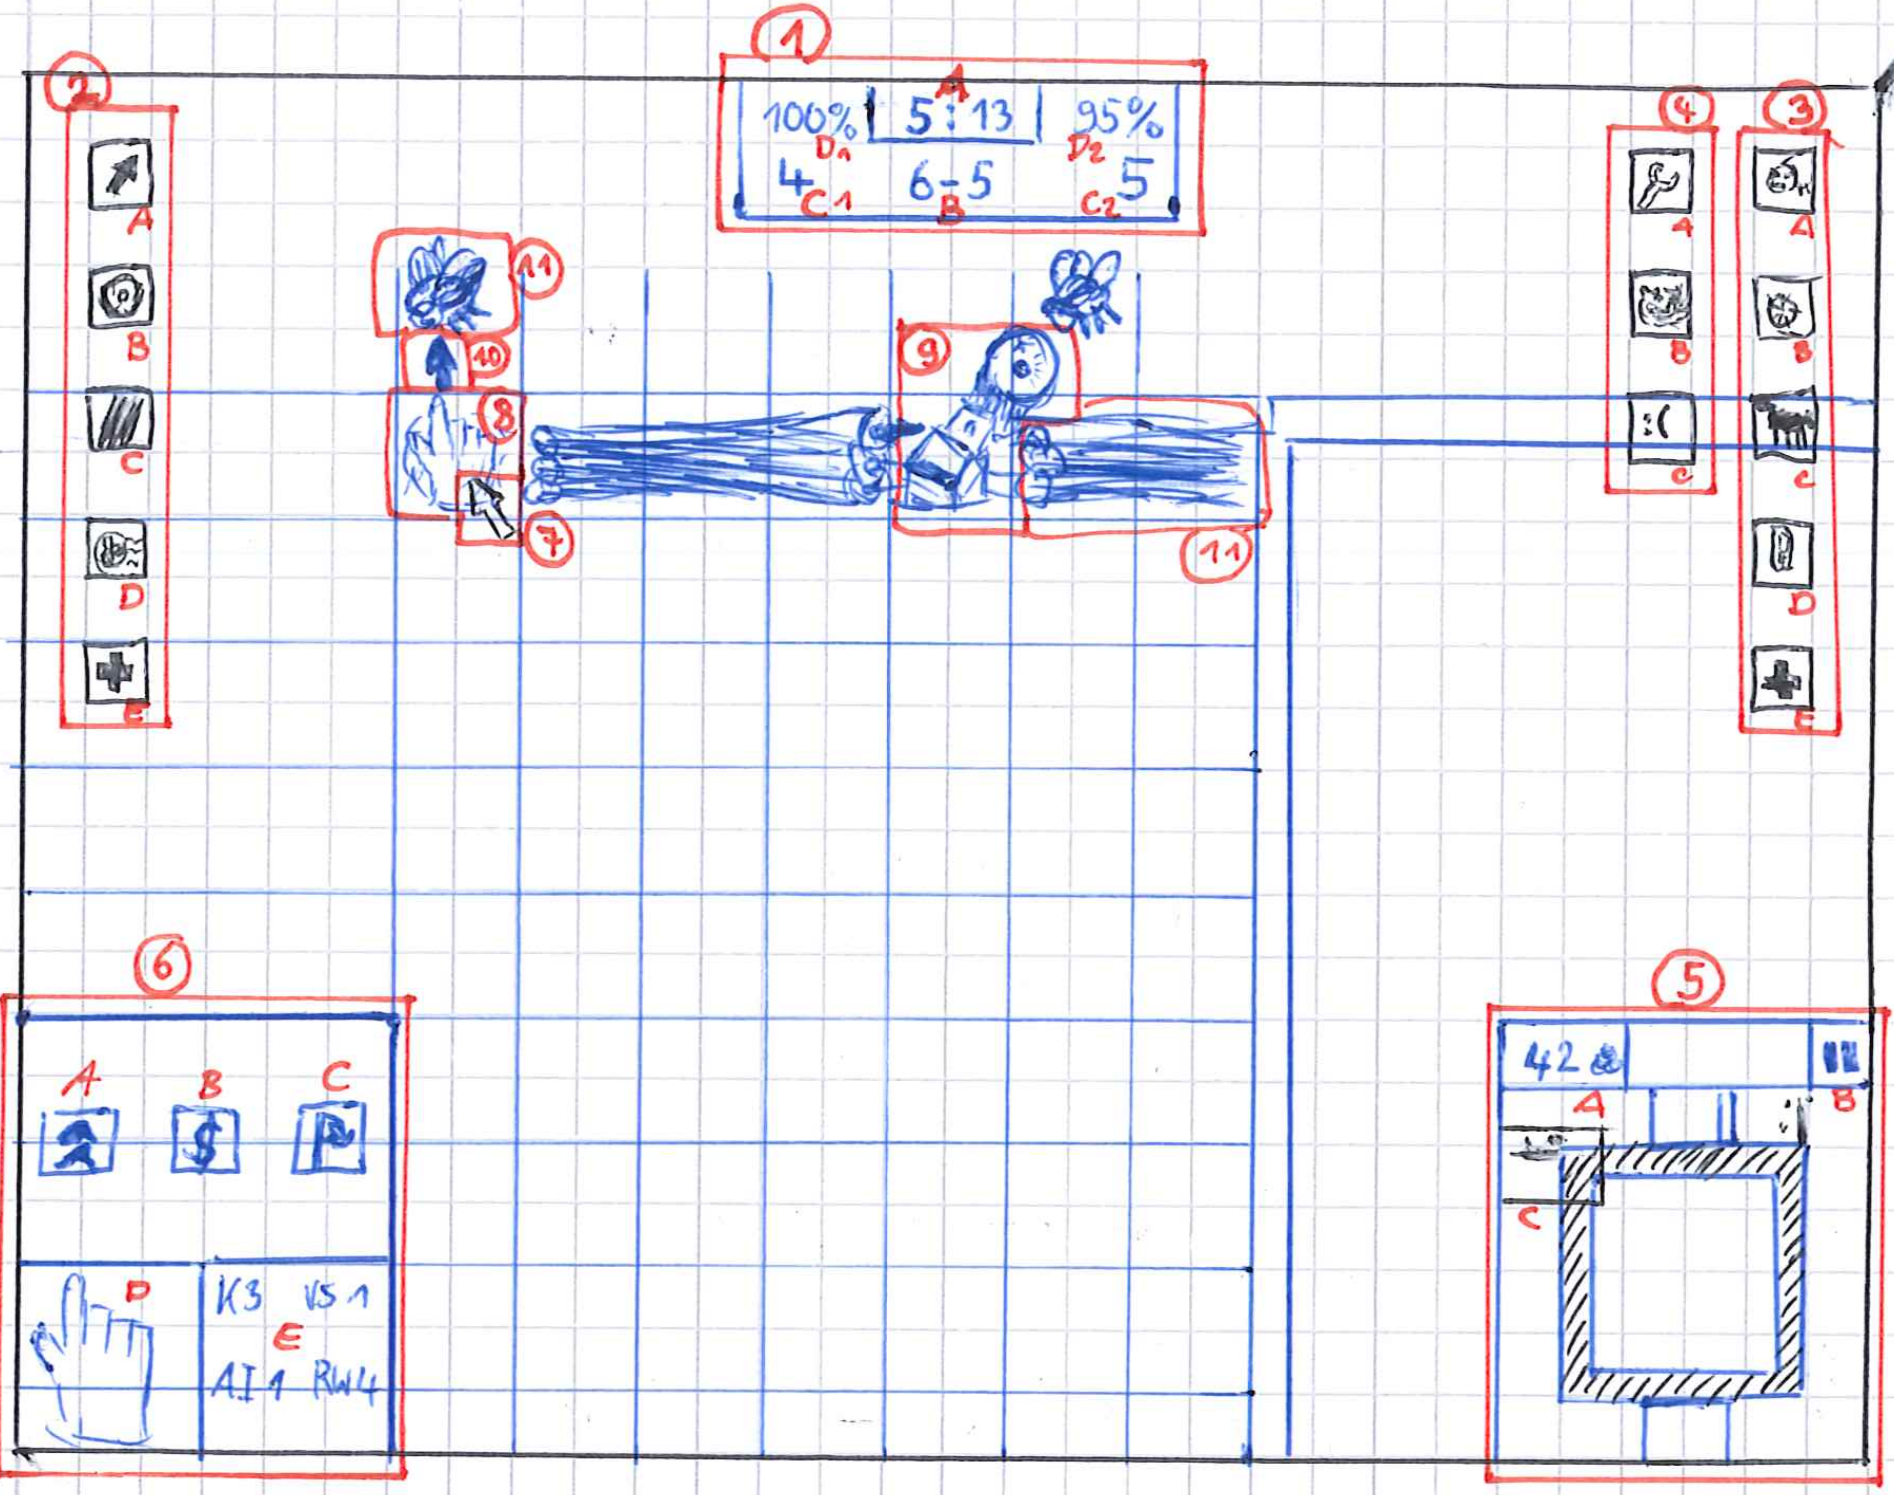
\includegraphics[width=1\textwidth]{spieler-interface.png}
	\caption{Spieler-Interface}
	\label{fig:spieler-interface}
\end{figure}


\section{Menü-Struktur}

% Siehe auch: https://sopra.informatik.uni-freiburg.de/soprawiki/Men%C3%BC

% Bei der Beschreibung der Menü-Struktur wird erklärt, wie das Hauptmenü und
% alle In-Game-Menüs zueinander in Beziehung stehen. Hilfreich dazu kann ein
% Diagramm in Form eines Graphen oder Baums sein.
%
% Wichtig ist, dass ersichtlich wird, welche Aktion im Menü welche Reaktion des
% Interfaces verursacht. Beispiel: "Wenn man im Einstellungsmenü auf 'Zurück'
% klickt, gelangt man zurück ins Hauptmenü."
%
% Ebenso wichtig ist die Vollständigkeit der Beschreibung. Jedes Menü und jedes
% Untermenü sollten erklärt werden.

\missingSection{Menü-Struktur}



\chapter{Technische Merkmale}

% Die technischen Merkmale beinhalten eine Übersicht über die unterschiedlichen
% Technologien, welche im Spiel verwendet werden.


\section{Verwendete Technologien}

% In diesem Abschnitt sollten alle verwendeten Technologien, die zur Erstellung
% des Spiels wichtig sind, stichpunktartig erwähnt werden. Das beinhaltet XNA
% ebenso wie eventuell verwendete externe Bibliotheken. Auch die Programme, die
% verwendet werden, um Modelle, Grafiken und Sounds zu erstellen werden hier
% erwähnt. Wenn zusätzliche Programme, wie zum Beispiel Physik Engines, vom
% Spiel vorausgesetzt werden, wird dies hier ebenso erwähnt.

\missingSection{Verwendete Technologien}

\begin{itemize}[leftmargin=*, nosep]
    \item Microsoft C\#
    \item Monogame 3.7
    \item Visual Studio Community 2019 mit ReSharper 2019.1
    \item Gitea
    \item Telegram
\end{itemize}


\section{Mindestvoraussetzungen}

% Dieser Abschnitt ist von der Form her vergleichbar mit den
% Mindestvoraussetzungen, die auf Spieleverpackungen gedruckt sind. Er
% beinhaltet die minimale Hardware, die notwendig ist, um das Spiel flüssig
% spielen zu können, sowie die benötigte Software und Bibliotheken. Um die
% Hardwarevoraussetzungen zu ermitteln, gibt es unterschiedliche Möglichkeiten:
%
%   • Die Hardwarespezifikationen des schlechtesten PCs eines Gruppenmitglieds,
%     auf dem das Spiel noch ohne Probleme läuft
%
%   • Die Ausstattung der Pool-Rechner (falls kein Gruppenmitglied einen PC hat,
%     auf dem das Spiel lauffähig ist)

\missingSection{Mindestvoraussetzungen}

\begin{itemize}[leftmargin=*, nosep]
    \item \dots
\end{itemize}



\chapter{Spiellogik}

% In diesem Abschnitt wird die gesamte Spielmechanik und alle im Spiel
% vorkommenden Spielobjekte erklärt. Sinn dieses Abschnittes ist es, eine
% Übersicht über alle Interaktionen des Spielers mit der Spielwelt und den
% Spielobjekten zu erhalten.

\todo[inline, caption = {Seitenumbrüche}]{%
  Wenn dieses Kapitels fertig ist, müssen evtl. Seitenumbrüche manuell
  eingefügt werden, um ein sinnvolles Ergebnis zu erzielen.}

\section{Spielobjekte}

% Hier sind alle Spielobjekte aufgelistet, die es im Spiel gibt. Dies können
% zum Beispiel Einheiten, Gebäude, Hindernisse usw. sein. Hilfreich zum
% Verständnis und zur Identifizierung der einzelnen Objekte können Bilder sein.
%
% Insbesondere erklärt dieser Abschnitt alle Eigenschaften und Fähigkeiten der
% unterschiedlichen Objekte. Sind sie zum Beispiel einfach zu zerstören, kosten
% sie viele Ressourcen, usw.
%
% Spielobjekte können hier auch schon mit konkreten Werten versehen werden;
% wenn noch keine konkreten Werte vorliegen (z.B. wie viele Lebenspunkte eine
% bestimmte Einheit hat), sollten zumindest die Verhältnisse der Werte von
% unterschiedlichen Spileobjekten aufgelistet werden, also zum Beispiel: Welche
% Einheit ist stärker als eine andere? Dass sich konkrete Werte noch verändern
% können, ist selbstverständlich, und eine Frage des Balancings gegen Ende des
% Projekts.

\missingSection{Spielobjekte}

\todo[inline, caption = {Seitenumbrüche}]{%
  Wenn der vorhergehende Teil des Kapitels fertig ist, müssen evtl.
  Seitenumbrüche manuell eingefügt werden, um ein sinnvolles Ergebnis zu
  erzielen.}

\subsection{Angriffseinheiten}

\begin{description}
  \item[Truppen]\todo[noline]{Benennung überdenken}
    kosten relativ wenig, lassen sich jedoch nicht weiter kontrollieren. Diese
    Einheiten verfolgen das Ziel, möglichst schnell zum gegenerischen Lager zu
    gelangen um dort Schaden zu verursachen.

  \item[Helden] kosten mehr als Truppen, diese Einheiten lassen sich jedoch vom
    Spieler kontrollieren und so strategisch einsetzen und außerhalb der
    Reichweite von Verteidigungsgebäuden positionieren; zusätzlich besitzen sie
    Fähigkeiten, die der Spieler einsetzen kann.

\end{description}

Tabelle~\ref{tab:attack-unit-props} beschreibt die Eigenschaften die
Angriffseinheiten haben, in Tabelle~\ref{tab:attack-units} sind alle Truppen
mit ihren Eigenschaften aufgelistet und Tabelle~\ref{tab:attack-heroes} enthält
alle Helden.

\begin{table}[htbp]
  \caption{Eigenschaften von Angriffseinheiten}
  \label{tab:attack-unit-props}
  \small
  \begin{longtabu}{rlX}
    \toprule\rowfont{\itshape}
    & Eigenschaft & Beschreibung \\
    \midrule

    B  & Beschreibung
       & Eine allgemeine Beschreibung dieser Einheit und Vergleich zu anderen
         Einheiten. \\
    F  & Fähigkeit
       & Nur Helden haben eine Fähigkeit, diese kann vom Spieler aktiviert
         werden (\refid{A:hero-ability}). \\
    K  & Kosten
       & Die Menge an Gold die aufgewendet werden muss, um eine dieser
         Einheiten zu kaufen (\refid{A:buy-attack}). \\
    LP & Lebenspunkte
       & Die Zahl der Lebenspunkte einer Einheit: Angriffe von
         Verteidigungstürmen ziehen Lebenspunkte von diesem Wert ab; fällt er
         unter Null, so stirbt diese Einheit (\refid{A:die}). \\
    AS & Angriffsstärke
       & Schaden, den diese Einheit am gegenerischen Lager verursacht, wenn sie
         dieses erreicht (\refid{A:damage-base}). \\
    GS & Geschwindigkeit & Distanz, die pro Zeiteinheit zurückgelegt werden
         kann. \\

    \bottomrule
  \end{longtabu}
  \todo[inline, caption = {Größe und Kollision}]{%
    Größe und Kollision evtl. in die Tabelle aufnehmen, aber was sagt die Größe
    genau aus? Diese ist doch nur interessant, wenn die Einheit kollidiert?}
\end{table}

\begingroup
  \small
  \begin{longtabu}{rXp{0.191\linewidth}}
    \rowfont{\normalsize}
    \caption{Truppen und ihre Werte\label{tab:attack-units}}
    \\\midrule[\heavyrulewidth]\endfirsthead

    % TODO: This seems to introduce too much vertical whitespace between the
    % midrule and the next row.
    \rowfont{\normalsize}
    \caption[]{Truppen und ihre Werte (fortges.)}
    \\\midrule[\heavyrulewidth]\endhead

    % TODO: At the moment this leads to strange page breaks, revisit when there
    % is more content!
    %
    % \multicolumn{3}{r}{\itshape fortges. auf der nächsten Seite}
    % \\\endfoot
    %
    % \endlastfoot

    \multicolumn{3}{c}{\bfseries Bug} \\*\midrule
    B  & Eine schnelle Sprintereinheit ohne viele Lebenspunkte, die alleine
         nicht besonders viel Schaden verursacht, aber in großer Masse gekauft
         werden kann, da sie nicht viel kostet.
       & \missingpic \\*
    K  & 1    \\*
    LP & 1    \\*
    AS & 1    \\*
    GS & 10   \\
    \midrule[\heavyrulewidth]

    \multicolumn{3}{c}{\bfseries Virus} \\*\midrule
    B  & Durchschnittliche Einheit, die etwas mehr kostet als ein \emph{Bug,}
         etwas langsamer ist, aber mehr LP hat und mehr Schaden verursacht.
       & \missingpic \\*
    K  & 2      \\*
    LP & 2      \\*
    AS & 2      \\*
    GS & 5      \\
    \midrule[\heavyrulewidth]

    \multicolumn{3}{c}{\bfseries Trojaner} \\*\nopagebreak\midrule\nopagebreak
    B  & Stirbt diese Einheit, werden an der Stelle ihres Todes \emph{Bugs} und
         \emph{Viren} gespawnt. Ein Trojaner ist zwar relativ langsam und kostet
         mehr als \emph{Viren,} hat dafür aber mehr LP und mehr AS.
       & \missingpic \\*
    K  & 4 \\*
    LP & 4 \\*
    AS & 4 \\*
    GS & 3 \\
    \midrule[\heavyrulewidth]

    \multicolumn{3}{c}{\bfseries Nokia} \\*\midrule
    B  & Diese Einheit ist bei gleichen Kosten zwar langsamer als ein
         \emph{Trojaner,} dafür aber hat sie mehr LP und AS.
       & \missingpic \\*
    K  & 4 \\*
    LP & 6 \\*
    AS & 6 \\*
    GS & 2 \\
    \midrule[\heavyrulewidth]

    \multicolumn{3}{c}{\bfseries Thunderbird} \\*\midrule
    B  & Diese Einheit fliegt, daher muss sie nicht den Weg um Mauern und Türme
         herumfinden, sondern kann einfach auf Luftlinie darüber hinwegfliegen.

         Von den Kosten ist diese Einheit mit \emph{Trojaner} vergleichbar, sie
         ist zwar etwas schneller, hat aber nicht viele LP und weniger AS.
       & \missingpic \\*
    K  & 4 \\*
    LP & 4 \\*
    AS & 3 \\*
    GS & 4 \\

    \bottomrule
  \end{longtabu}
  \missingpics{Bilder für Truppen}
\endgroup

\begingroup
  \small
  \begin{longtabu}{rXp{0.191\linewidth}}
    \rowfont{\normalsize}
    \caption{Helden und ihre Werte\label{tab:attack-heroes}}
    \\\midrule[\heavyrulewidth]\endfirsthead

    % TODO: This seems to introduce too much vertical whitespace between the
    % midrule and the next row.
    \rowfont{\normalsize}
    \caption[]{Helden und ihre Werte (fortges.)}
    \\\midrule[\heavyrulewidth]\endhead

    % TODO: At the moment this leads to strange page breaks, revisit when there
    % is more content!
    %
    % \multicolumn{3}{r}{\itshape fortges. auf der nächsten Seite}
    % \\\endfoot
    %
    % \endlastfoot

    \multicolumn{3}{c}{\bfseries Settings} \\*\midrule
    B  & Diese Einheit heilt Truppen um sich herum, hat jedoch selbst
         eher wenig LP; diese ist die langsamste der Heldeneinheiten, sie
         verursacht am gegenerischen Lager keinen Schaden.
       & \missingpic \\*
    F  & \emph{(passiv)} heilt verbündete Truppen in einem gewissen Radius
         regelmäßig um einen Wert (\refid{H:heal}).\\*
    K  & 10   \\*
    LP & 4    \\*
    AS & 0    \\*
    GS & 4    \\
    \midrule[\heavyrulewidth]

    \multicolumn{3}{c}{\bfseries Firefox} \\*\midrule
    B  & Dieser Held ist eine starke Angriffseinheiten, die mit ihrer Fähigkeit
         leichter zwischen den Verteidigungsgebäuden hindurchkommt. Der
         \emph{Firefox} ist relativ schnell, hat durchschnittliche LP und
         relativ viel~AS.
       & \missingpic \\*
    LP & 6      \\*
    AS & 8      \\*
    GS & 8      \\*
    K  & 10     \\*
    F  & \emph{(aktiv)} kann Verteidigungsgebäude überspringen
         (\refid{H:jump}).\\
    \midrule[\heavyrulewidth]

    \multicolumn{3}{c}{\bfseries Bluescreen} \\*\nopagebreak\midrule\nopagebreak
    B  & Diese Einheit unterstützt verbündete Einheit, indem sie gegenerische
         Verteidigungsgebäude für einen Moment deaktivieren kann; dafür
         verursacht sie am gegenerischen Lager selbst keinen Schaden, hat wenige
         LP ist aber schnell.
       & \missingpic \\*
    LP & 4      \\*
    AS & 0      \\*
    GS & 10     \\*
    K  & 10     \\*
    F  & \emph{(aktiv)} kann eine Schockwelle zünden, um gegenerische
         Verteidigungsgebäude in der Nähe für einen Moment zu deaktivieren
         (\refid{H:emp}).

         Um diese Fähigkeit erneut einzusetzen, muss diese Einheit zur Basis
         zurückkehren um sich aufzuladen (\refid{H:reload}).\\

    \bottomrule
  \end{longtabu}
  \missingpics{Bilder für Helden}
\endgroup


\subsection{Verteidigungsgebäude}

In Tabelle~\ref{tab:defend-props} werden die Eigenschaften von
Verteidigungsgebäuden beschrieben, Tabelle~\ref{tab:defend-units} enthält die
Gebäude und weist den Eigenschaften Werte zu. Der Wert W berechnet sich aus der
Menge an Bitcoin, die in dieses Gebäude investiert wurde.

Im Laufe des Spiels kann der Spieler folgende Aktionen auf eigenen Türmen
ausführen:

\begin{description}
  \item[Verkaufen] (\refid{A:tower-sell}) Das Gebäude verschwindet, es können
    neue Gebäude an dieser Stelle gebaut werden und feindliche Einheiten können
    wieder über diese Felder laufen.

    Der Spieler erhält 80\,\% des Gebäudewertes an Bitcoin.

  \item[Verbessern] (\refid{A:tower-improve}) Erhöht die Reichweite des
    Gebäudes (außer bei \emph{Schockfeld}) um 50\,\% des aktuellen Wertes und
    reduziert das Angriffsintervall um 20\,\% des aktuellen Wertes.

    Die Verbesserung kostet den Spieler 50\,\% des aktuellen Turmwertes und der
    Turmwert steigt um diese Kosten.

    Bei \emph{Kabel} ist keine Verbesserung möglich, jedes andere Gebäude kann
    maximal zweimal verbessert werden.

  \item[Strategie wählen] (\refid{A:tower-strategy}) Mögliche Strategien sind
    \begin{description}[itemsep=0pt]
      \item[Erste Einheit] \emph{(ist standardmäßig ausgewählt)}\\
        Greift die Einheit an, die den kürzesten Weg hat, um Schaden an der Basis
        zu verusachen.

      \item[Stärkste Einheit] ~\\
        Greift die Einheit an, die die meisten LP hat.

      \item[Schwächste Einheit] ~\\
        Greift die Einheit an, die die wenigsten LP hat.
    \end{description}

    Bei \emph{Kabel} und \emph{Schockfeld} ist ein wählen der Strategie nicht
    möglich.

\end{description}


\begingroup
  \small
  \begin{longtabu}{rlX}
    \rowfont{\normalsize}
    \caption{Eigenschaften von Verteidigungsgebäuden\label{tab:defend-props}}\\

    \midrule[\heavyrulewidth]\rowfont{\itshape}
    & Eigenschaft & Beschreibung \\
    \midrule

    B  & Beschreibung
       & Eine allgemeine Beschreibung dieser Einheit und Vergleich zu anderen
         Einheiten. \\
    K  & Kosten
       & Die Menge an Bitcoin die aufgewendet werden muss, um eines dieser
         Gebäude zu platzieren~(\refid{A:put-defend}). \\
    VS & Verteidigungsstärke
       & Schaden, den dieses Gebäude an getroffenen Gegner
         verursacht~(\refid{A:unit-hit}). \\
    AI & Angriffsintervall
       & Zeit die vergehen muss, bevor dieses Gebäude erneut Gegner angreifen
         kann~(\refid{A:tower-attack}). \\
    RW & Reichweite
       & Radius um den Turm, in dem Einheiten angegriffen werden können, und in
         dem die Effekte der Türme auf die Einheiten wirken. \\

    \bottomrule
  \end{longtabu}
\endgroup

\begingroup
  \small
  \begin{longtabu}{rXp{0.191\linewidth}}
    \rowfont{\normalsize}
    \caption{Verteidigungsgebäude und ihre Werte\label{tab:defend-units}}
    \\\midrule[\heavyrulewidth]\endfirsthead

    \rowfont{\normalsize}
    \caption[]{Verteidigungsgebäude und ihre Werte (fortges.)}
    \\\midrule[\heavyrulewidth]\endhead

    \multicolumn{3}{r}{\itshape fortges. auf der nächsten Seite}
    \\\endfoot

    \endlastfoot

    \multicolumn{3}{c}{\bfseries Kabel} \\*\midrule
    B  & Dieses Gebäude kostet wenig, steht gegnerischen Einheiten im Weg und
         verursacht keinen Schaden.
       & \missingpic \\*
    K  & 2 \\*
    VS & --- \\*
    AI & --- \\*
    RW & --- \\
    \midrule[\heavyrulewidth]

    \multicolumn{3}{c}{\bfseries Mauszeigerschütze} \\*\midrule
    B  & Durchschnittlicher Verteidigungsturm, der Mauszeiger auf ein
         Einzelziel verschießt.
       & \missingpic \\*
    K  & 3 \\*
    VS & 1 \\*
    AI & 1 \\*
    RW & 4 \\
    \midrule[\heavyrulewidth]

    \multicolumn{3}{c}{\bfseries CD-Werfer} \\*\midrule
    B  & Dieser Turm kostet mehr und schießt langsamer als ein
         \emph{Mauszeigerschütze,} dafür verursacht das Projektil (die CD)
         jedoch auf ihrem Weg an jedem berührten Gegner den Schaden der Höhe
         VS.
       & \missingpic \\*
    K  & 5 \\*
    VS & 4 \\*
    AI & 3 \\*
    RW & 3 \\
    \midrule[\heavyrulewidth]

    \multicolumn{3}{c}{\bfseries Antivirusprogramm} \\*\midrule
    B  & Von den Kosten ist dieser Turm vergleichbar zum \emph{CD-Werfer,}
         allerdings schießt das \emph{Antivirusprogramm} noch langsamer,
         verursacht dafür aber an einem Einzelziel erheblichen Schaden.
       & \missingpic \\*
    K  & 5 \\*
    VS & 7 \\*
    AI & 5 \\*
    RW & 6 \\
    \midrule[\heavyrulewidth]

    \multicolumn{3}{c}{\bfseries Lüftung} \\*\midrule
    B  & Dieser Turm verlangsamt alle Einheiten im Einflussbereich.
       & \missingpic \\*
    K  & 5 \\*
    VS & 7 \\*
    AI & 5 \\*
    RW & 4 \\
    \midrule[\heavyrulewidth]

    \multicolumn{3}{c}{\bfseries Wifi-Router} \\*\midrule
    B  & Dieser Turm schießt nahezu dauerhaft kreisförmige Wellen, die wenig
         Schaden verursachen und Gegner penetrieren.
       & \missingpic \\*
    K  & 5 \\*
    VS & 2 \\*
    AI & 1 \\*
    RW & 5 \\
    \midrule[\heavyrulewidth]

    \multicolumn{3}{c}{\bfseries Schockfeld} \\*\midrule
    B  & Dieses „Gebäude“ blockiert die Gegner nicht, sie laufen darüber
         hinweg. In regelmäßigen Abständen erhalten alle Gegner schaden, die
         auf einem \emph{Schockfeld} sind.
       & \missingpic \\*
    K  & 4 \\*
    VS & 2 \\*
    AI & 3 \\*
    RW & 0 \\

    \bottomrule
  \end{longtabu}
  \missingpics{Bilder für Verteidigungsgebäuden}
\endgroup


\subsection{Sonstige}

\begin{description}
  \item[Computer] \todo[noline]{Bezeichnung in Ordnung?}
    Ein Computer hat eine Ladung, zu Beginn ist diese bei 100\,\%. Jede
    feindliche Angriffseinheit, die den Computer erreicht, zieht von der Ladung
    so viele Prozent ab, wie die Einheit AS hat. Fällt die Ladung auf 0\,\% oder
    einen negativen Wert, so geht dieser Computer aus (\refid{A:base-die}).
    \todo{Alternative Formulierung: \emph{kaputt}}

  \item[Spieler]

  \item[Gegner]
\end{description}


\section{Optionen und Aktionen}

% Siehe auch: https://sopra.informatik.uni-freiburg.de/soprawiki/Game_Mechanic

% Dieser Abschnitt beinhaltet die Aktionen, die Spieler oder KI vornehmen
% können, um den Zustand des Spiels zu verändern (zB das Bauen von Einheiten
% oder das Abbauen von Ressourcen). Je klarer diese Aktionen formuliert sind,
% desto leichter fällt einem die Umsetzung der Aktionen bei der Programmierung
% des Spiels.
%
% Wichtig sind auch die Einstellungen, die der Spieler am Spiel vornehmen kann,
% um das Spielverhalten zu verändern (zB.  Schwierigkeitsgrad ändern).
%
% Das Ziel des Spiels sollte schließlich anhand der beschriebenen Aktionen
% erklärt werden.
%
% Die Auflistung der Optionen und Aktionen erfolgt tabellarisch und ist in Form
% und Inhalt an Use Cases (http://de.wikipedia.org/wiki/Use_case) angelehnt.

\missingSection{Optionen und Aktionen}

\begin{table}[h]
  \caption{Mögliche Optionen und Aktionen}
  \small
\begin{longtabu}{X[0.6L]X[0.4L]X[L]X[0.9L]X[0.9L]}
  \toprule
  \rowfont{\itshape}
    ID/Name              &
    Akteure              &
    Ereignis"-fluss      &
    Anfangs"-bedingung   &
    Abschluss"-bedingung \\
  \midrule\endhead

  % Example line taken from the SOPRA wiki.
  ID01: Figur durch Klick bewegen
    & Spieler
    & \dots
    & Der Spieler muss eine oder mehr kontrollierbare, auswählbare Spielfiguren
      ausgewählt haben.
    & Die Spielfiguren befinden sich am Zielpunkt, \textbf{oder} die
      Spielfiguren befinden an einem begehbaren Punkt in der Welt, der möglichst
      nah am Ziekpunkt liegt.
  \\

  \bottomrule
\end{longtabu}
\end{table}


\section{Spielstruktur}

% Dieser Abschnitt erklärt den Ablauf des Spiels. Das heißt, hier wird
% beschreiben, was geschieht, sobald der Spieler ein neues Spiel beginnt und
% wie sich das Spiel von dort aus entwickelt, bis es gewonnen oder verloren
% ist. Eine Beschreibung der unterschiedlichen Spielphasen ist hier essentiell.
%
% Eine mögliche Einteilung der Spielphasen von Schach ist zum Beispiel:
% Early-Game (Eröffnung), Mid-Game (strategische Positionen festigen),
% Late-Game (wenn nur noch wenige Figuren auf dem Brett sind).
%
% Eine weitere wichtige Information in diesem Abschnitt ist, welche Modi das
% Spiel hat (zum Beispiel Missionen und wie sie sich unterscheiden vs.
% Endlosmodus und wie dieser während des Spiels verändert wird).
%
% Außerdem soll die Dynamik des Spiels beschrieben werden (Beispiel: statisch,
% d.h. wenig Veränderungen an der Spielwelt und den Mechaniken vs. actionreich
% und dynamisch).
%
% Auch mögliche Taktiken und Strategien im Spiel können hier beschrieben
% werden.

Das Spiel ist ein dynamisches Spiel. 

\subsection{Kaufoptionen}
\label{subsec:kaufoptionen}
    Alle Angriffs- und Verteidigungseinheiten, deren Verbesserungen und deren
    Upgrades können zu jedem Zeitpunkt während des Spiels gekauft werden, 
    solange genug Bitcoin vorhanden ist. Unterschiede bestehen beim 
    Aktivierungszeitpunkt.

	\begin{enumerate}
		\item Verbesserungen: Die Veränderung tritt sofort in Kraft.
		\item Upgrades: Die Veränderung tritt sofort in Kraft.
    		\item Kaufen neuer Einheiten
		\begin{enumerate}
			\item Türme: Sobald der gewählte Platz leer ist wird
				gebaut.
			\item Angriffseinheiten: Käufe bildet die Angreifer 
				für die nächste Welle.
    		\end{enumerate}
	\end{enumerate}

\subsection{Spielablauf}
Beim Starten eines neuen Spiels erscheint ein Feld mit der
Hintergrundgeschichte. Hier wird kurz in die Idee hinter der Spielwelt
eingeführt. //
Wenn das Feld geschlossen landet man bei der ersten Spielwelt. Jetzt hat der 
Spieler Zeit die erste Welle vorzubereiten, sprich seine Türme aufzustellen 
und seine Angriffseinheiten zu kaufen. Dafür hat der Spieler 50 Einheiten Bitcoin
zur Verfügung. //
Nun kann die erste Welle gestartet werden.
Nun laufen die Angriffseinheiten in kurzen Abständen hintereinander von der
eigenen Basis los, auf die gegnerischen Türme zu. Die Reihenfolge entspricht
der Kaufreihenfolge. Zusätzlich tauchen die drei kontrollierbaren,
kollidierenden und bewegbaren Einheiten (Helden) am Ausgang der Basis auf. Diese
können von nun an mit der Maus gesteuert werden. \\
Sobald das Spiel gestartet wird verdient der Spieler über Zeit Bitcoin. Dieses
kann auch sofort wieder investiert werden. Für jeden Bitcoin besteht die
Wahl zwischen Angriff und Verteidigung(\ref{subsec:kaufoptionen}). \\

Die nächste Welle wird gestartet sobald einer der beiden Spieler keine 
Angriffseinheiten, mit Ausnahme der Helden, mehr auf dem Spielfeld besitzt
und beide Basen noch Leben besitzen. Die verbliebenen Einheiten des zweiten 
Spielers attakieren weiter bis sie ebenfalls tot sind. \\
Sobald die gesamte Angriffseinheit, mit Ausnahme der Helden, tot ist oder die 
gegnerische Basis erreicht hat, bekommt dieser Spieler einen Erfahrungspunkt. 
Außerdem bekommt der Spieler mit der höheren Anzahl an Angreifern die 
Differenz der Anzahl der Angreifer der beiden Spieler in Bitcoin gut geschrieben.
Die Höhe dieses Betrags ist jedoch pro Welle limitiert und das Limit steigt 
mit zunehmender Anzahl an Wellen an.\\

Dieser Prozess wiederholt sich solange bis einer der beiden Basen zerstört 
wurde. Der Spieler, der die Basis zerstört hat, gewinnt das Spiel. 
Jetzt erscheint ein Gewonnen oder Verloren Bildschirm vom dem in das Hauptmenü
zurück gekehrt werden kann.


\section{Statistiken}

% Statistiken erlauben es einem Spieler, sich mit anderen Spielern zu messen
% und zu entscheiden, wer besser ist und sind ein wichtiger Bestandteil von
% nahezu jedem Spiel.
%
% In diesem Abschnitt wird erklärt, welche unterschiedlichen Statistiken
% während des Spiels gesammelt werden, wie sie Einfluss auf das Spielgeschehen
% geben und wodurch die unterschiedlichen Werte während des Spiels geändert
% werden.
%
% Das einfachste Beispiel für Statistiken sind Highscore-Listen, in denen die
% größte erreichte Punktzahl eines Spieldurchlaufs pro Spieler aufgelistet ist.

\emph{Kernel Panic!} sammelt für jeden Spieldurchlauf die folgenen Statistiken:

\begin{itemize}[noitemsep, leftmargin=*]
	\item Sieger-Seite
	\item Dauer der Spielzeit
	\item APM (actions per minute)
	\item Anzahl besiegter gegnerischer Einheiten / Total Damage dealt
	\item Bitcoin investiert in Angriffseinheiten
	\item Bitcoin investiert in Verteidigungsgebäude
	\item Bitcoin investiert in Upgrades
	\item Bitcoin investiert in Special-Upgrades
	\item Zusätzlich erworbene Bitcoins (Wie viel Bitcoin hat man durch Bauen von Einheiten zusätzlich erworben)
\end{itemize}

%\missingSection{Statistiken}


\pagebreak
\section{Achievements}

% In diesem Abschnitt werden die unterschiedlichen Achievements und die
% Bedingungen, wie diese erreicht werden können, aufgelistet.
%
% Achievements können verschiedene Schwierigkeitsstufen besitzen, um sie zu
% erreichen. Achievements mit unterschiedlichen Schwierigkeitsstufen sind z.B.:
% "Zerstöre 2000 gegnerische Einheiten" vs. "Schaffe das gesamte Spiel, ohne
% einen Schuss abzufeuern".

Tabelle~\ref{tab:achievements} beschreibt die Achievements in \emph{Kernel Panic!.}
\begingroup
  \small
  \tabulinesep=1.2mm
  \begin{longtabu}{X[0.7]X}
    \rowfont{\normalsize}
    \caption{Mögliche Achievements in \emph{Kernel Panic!}\label{tab:achievements}}\\
    \midrule[\heavyrulewidth]\rowfont{\itshape}
    Name & Beschreibung \\
    \midrule\endfirsthead

    \rowfont{\normalsize}
    \caption[]{Achievements (fortges.)}\\
    \midrule[\heavyrulewidth]\rowfont{\itshape}
    Name & Beschreibung \\
    \midrule\endhead

    \bottomrule
    \multicolumn{2}{r}{\emph{fortges. auf der nächsten Seite}} \\
    \endfoot

    \endlastfoot

    % Example
    First Victory! / GG EASY / Is Dis Tetris?
      & Du hast das Spiel zum 1./10./100. Mal gewonnen!
      	\\
    Unlucky Loss / Rekt / Complete Humiliation
    	& Du hast das Spiel zum 1./10./100. Mal verloren
    	\\
	Minion Slayer
		& Du hast in einem Spiel X Angriffseinheiten getötet
		\\
	Bitcoin Addiction
		& Du besitzt in einem Spiel über X Bitcoin
		\\
	while true DO sudo apt-get upgrade DONE
		& Du hast in einem Spiel über X Bitcoin in Upgrades investiert
		\\
	Iron Fortress
		& Du gewinnst das Spiel mit einer Ladung von 100\%
		\\
	Tower's win the game
		& Du hast in einem Spiel über X Bitcoin in Verteidigungsgebäude investiert
		\\
	Bitcoin Thief
		& Du hast in einem Spiel über X Bitcoin zusätzlich durch Überqueren des gegnerischen
		Territoriums erbeutet
		\\
	Bank Account Hacked!
		& Dein Gegner hat in einem Spiel über X Bitcoin zusätzlich durch Überqueren deines
		Territoriums erbeutet
		\\
	Dirty Coder
		& Du hast in einem Spiel über X Bug-Einheiten gebaut
		\\
	Fix your Code!
		& Du hast in einem Spiel über X Bug-Einheiten besiegt
		\\
	Bzzzz
		& Du hast in einem Spiel X Einheiten mit Schockfeld besiegt
		\\
	APM God
		& Du hast in einem Spiel über X APM
		\\
	Idle Gamer
		& Du hast in einem Spiel über X Runden nichts gebaut/abgerissen oder Bitcoin in upgrades investiert
		\\
	Hacker
		& Du hast in einem Spiel über X Virus-/Trojaner-Einheiten gebaut
		\\
	High Security Anti-Virus
		& Du hast in einem Spiel über X Virus-/Trojaner-Einheiten besiegt
		\\
	\st{Tower Defense} Jump 'n' Run
		& Du hast in einem Spiel X Verteidigungsgebäude mit der Firefox-Einheit übersprungen
		\\
	Fool!
		& Du hast versucht einen leeren Spielstand zu laden.
		\\
	Nutcracker
		& Du hast eine Nokia-Einheite besiegt.
		\\
	Teure Leitung
		& Du hast X viele Kabel-Einheiten gebaut
		\\
	High Inference
		& Gewinne nur mit Wifi-Router als Verteidigungsgebäude
		\\
    \bottomrule
  \end{longtabu}
\endgroup



\chapter{Screenplay}

% Dieser Abschnitt beinhaltet die Hintergrundgeschichte (Story) des Spiels.
% Eine Story ist wichtig für ein Spiel, um zu erklären, warum bestimmte
% Aktionen durchgeführt werden können, oder nicht. Eine Story ist auch ein
% einfacher Weg, um eine Umgebung zu schaffen, mit der sich ein Spieler
% identifizieren kann und Spaß daran hat, die Umgebung zu erforschen und sich
% darin zu bewegen.

\missingChapter{Screenplay}

\section{Konzeptzeichnungen \& Storyboards}

% Bilder sind wichtig für den ersten Eindruck. Vor allem im GDD sind
% Konzeptzeichnungen und Skizzen gut aufgehoben. Auf diese Weise kann man nicht
% nur sich selbst schnell eine Vorstellung von den Ideen machen, sondern auch
% anderen vermitteln, worum es im Spiel geht und wie das Spiel und seine
% Geschichte aussieht.

\missingSection{Konzeptzeichnungen \& Storyboards}



\end{document}
